\chapter{Desenvolupament}
Un cop vist com funciona el protocol del Bluetooth Low Energy, en aquest capítol s'analitzarà el dispositiu que l'implementa.
S'explicarà tant els components i parts que formen part del circuit imprès (\textit{Printed Circuit Board} o PCB d'ara endavant) com el programari que s'utilitza per desenvolupar projectes utilitzant-la.

\section{LaunchXL CC1352R1}
Per analitzar el protocol BLE i veure les seves característiques s'ha utilitzat el kit LaunchXL pel desenvolupament ràpid del microcontrolador CC1352R1.

\begin{figure}[h!]
	\begin{center}
		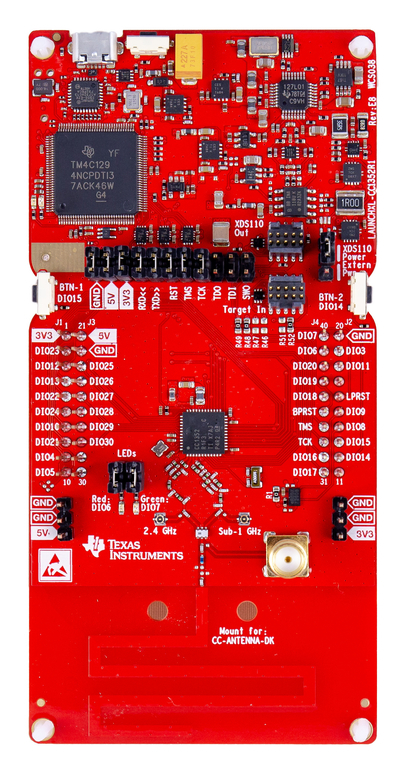
\includegraphics[width=0.5\textwidth]{./images/launchxl-cc1352r1.jpg}
		\caption{PCB amb la que es realitza el treball \cite{placa}}
		\label{PCB}
	\end{center}
\end{figure}

Aquesta PCB, que es pot veure a la figura \ref{PCB}, permet el desenvolupament d'aplicacions en BLE utilitzant el microcontrolador CC1352 de Texas Instruments.
A continuació es descriuen les seves característiques principals \cite{placa_datasheet}.

El dispositiu CC1352R és multiprotocol i multibanda orientat a 2.4 GHz o sub-1GHz que serveix per a Thread, Zigbee, Bluetooth 5 Low Energy, IEEE 802.15.4g i 6LoWPAN.
Pel que fa a memòria, té 352 KB flash programable, 256 KB de ROM per a protocols i llibreries, 8 KB de Cache SRAM i 80 KB de RAM protegida amb paritat.
D'els perifèrics el més important és l'ADC de 12 bits i 8 canals amb freqüència de mostreig de 200 Kmostres/s (multiplexat). També té Rellotge de Temps Real (RTC en anglès), acceleradors d'operacions criptogràfiques i generador de números aleatoris.
La radio multibanda que té un receptor amb sensibilitat de -121 dBm per a sub-1GHz i de -110 dBm a 50 Kbps o -105 dBm a 125 Kbps. El transmissor pot transmetre fins a 14 dBm sub-1GHz i 5dBm a 2.4 GHz.


\section{Software}
Pel desenvolupament de projectes per a la PCB s'ha utilitzat l'entorn de desenvolupament Code Composer Studio 9. 
El CCS el distribueix Texas Instruments i està basat en Eclipse \cite{eclipse}, que és de codi obert.
Aquest entorn de desenvolupament està orientat al desenvolupament per a processadors incrustats (\textit{embedded} en anglès) de les famílies fabricades per Texas Instruments.
El gran benefici d'aquest programa és que permet la depuració de programes basats en JTAG que és el cas d'aquesta PCB.

Texas Instruments té la plataforma SimpleLink que conté tant les llibreries necessàries per desenvolupar projectes com els recursos necessaris per a l'aprenentatge de les tecnologies que es volen implementar.
Per poder dur a terme projectes amb la PCB d'aquest treball és necessari utilitzar el SimpleLink CC13X2 versió 2.30.00.45\footnote{La versió utilitzada no és la més nova perquè sigui compatible amb la revisió C del xip que s'està utilitzant.}.

\section{Project 0}
El Project 0 és el projecte instal·lat amb què les PCB vénen de fàbrica.
Aquest projecte exposa certs serveis a través de BLE i permet fer una comunicació simple entre la PCB i un dispositiu mòbil.
Aquesta comunicació és bidireccional, és a dir, des del mòbil es poden controlar els LEDs que té la PCB.
I en el mòbil es pot veure si qualsevol dels dos botons està pitjat.

Aquest projecte serveix per tenir un bon exemple de com està dissenyada l'arquitectura dels serveis amb les seves característiques amb una relativa simple funcionalitat. A continuació s'analitzaran diferents parts dels atributs.

\subsection{Serveis de Botons i LEDs}

En la taula \ref{tab:project_zero_uuid} es poden veure els valors que hi ha tal com estan en la taula d'atributs del servidor GATT del Project 0.
Per facilitar la visualització de les dades s'han tret els zeros finals dels UUID propis però cal recordar que en total tenen 16 parells de caràcters (128 bits en representació hexadecimal) i no només els 9 parells que surten a la taula.
\begin{table}[h!]
	\begin{center}
		\csvautotabular{data_files/projectzeroUUID.csv}
		\caption{Atributs del Project 0}
		\label{tab:project_zero_uuid}
	\end{center}
\end{table}
Els atributs en si no es poden identificar per tant és necessari tenir en compte la documentació del Project 0.
En la documentació hi ha inclosa una taula on es relaciona cada UUID amb el corresponent significat que es pot observar a la figura \ref{project0_table}.

\begin{figure}[h!]
	\begin{center}
		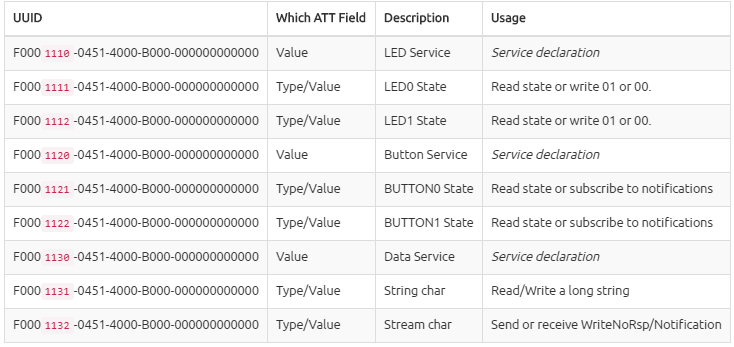
\includegraphics[width=\textwidth]{./images/Project_0_UUID.png}
		\caption{Definició dels UUID \cite{project0_UUIDs}}
		\label{project0_table}
	\end{center}
\end{figure}

El primer que cal tenir clar és que a la taula \ref{tab:project_zero_uuid} els valors estan representats amb l'ordre en què es reben i en general els serveis estandarditzats (i també aquest servei propi) utilitzen \textit{little-endian} per enviar la informació.
Això resulta en el fet que els caràcters hexadecimals queden (per parelles, ja que, dos caràcters representen un byte) ordenats al revés.

En analitzar els atributs es pot veure com aquells que tenen l'UUID 0x2800 (que corresponen a declaracions de serveis) en el seu valor únicament contenen l'UUID corresponent a les definicions de serveis de LEDs i de botons de la figura \ref{project0_table}.
Seguidament, als atributs amb UUID 0x2803 hi ha les definicions de les característiques, en el seu valor hi ha múltiples parts.
El primer parell hexadecimal (0x0E o 0x12, en aquest cas) correspon a les propietats.
Que defineixen l'accés a l'atribut que el succeeix.
Just després hi ha dos parells hexadecimals que identifiquen el \textit{Handle} de l'atribut on hi ha la característica.
Per últim, la resta de caràcters corresponen al UUID que identifica quina característica és.

\subsection{Propietats}
\label{sec:properties}
Les propietats d'accés són un valor que identifica quines operacions i procediments es poden fer sobre la característica.
Es poden veure les propietats principals amb els corresponents valors en la taula \ref{properties}.
El camp té 8 bits per defecte i cada un d'ells identifica una operació o procediment.
Es pot utilitzar qualsevol combinació d'aquests bits  per habilitar les opcions d'accés que es desitgin.

\begin{table}[h]
	\begin{center}
		\begin{tabular}{|c|c|l|}
			\hline
			Binary	&	Hex		&	Property	\\	\hline
			0000 0001	&	0x01	&	Broadcast\\	\hline
			0000 0010	&	0x02	&	Read	\\	\hline
			0000 0100	&	0x04	&	Write w/o Response	\\	\hline
			0000 1000	&	0x08	&	Write	\\	\hline
			0001 0000	&	0x10	&	Notification w/o ACK	\\	\hline
			0010 0000	&	0x20	&	Indication with ACK	\\	\hline
			0100 0000	&	0x40	&	Signed Writes	\\	\hline
			1000 0000	&	0x80	&	Aditional Properties	\\	\hline
		\end{tabular}		
	\end{center}
\caption{Valors de les propietats}
\label{properties}
\end{table}

Primer de tot, cal destacar la implementació de comunicacions amb reconeixement o sense. D'aquesta manera si es prefereix reduir la quantitat de missatges per estalviar energia en lloc d'assegurar-se que s'ha rebut la informació es dóna l'opció de no tenir reconeixements.

En el Project 0 les propietats de les característiques dels LEDs tenen el valor 0x0E que suposa  0000 1110 en binari, per tant, es permet: llegir, escriure i escriure sense resposta.
En canvi les característiques del servei de botons tenen el valor 0x12 que suposa 0001 0010, per tant, es permet la lectura i la notificació sense reconeixement.

La notificació i la indicació són funcions que ajuden a reduir el consum de recursos.
Quan es vol saber en quin estat estan els botons de la PCB contínuament es podria anar llegint l'estat de la característica constantment però això suposarien molts missatges i reduiria el temps que els dispositius es poden estalviar energia apagant la ràdio.
Per evitar aquest cas, es pot configurar la característica tal que sigui la mateixa PCB qui enviï el missatge automàticament quan l'estat de la característica canviï.
D'aquesta manera el receptor només cal que escolti els missatges de la PCB per tal de saber en quin estat està el botó.

En cas que es vulgui indicació amb reconeixements és possible configurar-ho d'aquesta manera a través de l'atribut Configuració de Característica del Client identificat amb l'UUID 0x2902 i estandarditzat en l'especificació de Bluetooth.
Si el valor és 0, no hi ha transmissions; si el valor és 1, s'envien notificacions (sense reconeixement) i si el valor és 2, s'envien indicacions (notificacions amb reconeixement). 

El bit d'extensió de propietats, en cas que sigui 1 indica que existeix l'atribut: Descriptor Propietats Esteses de Característica.
Aquest atribut té l'UUID 0x2900 i permet afegir més propietats de les que poden existir amb l'espai limitat de 8 bits que hi ha per defecte.
Aquest sistema permet afegir fins a 16 bits més per indicar propietats, actualment els dos primers es defineixen segons l'estàndard i la resta estan reservats per a ús futur \cite{extended properties}.

Aquests 2 primers que estan definits són escriptura fiable i escriptura auxiliar.
L'escriptura fiable permet escriure valors amb un procediment diferent de l'habitual que permet assegurar-se que el valor que es vol modificar s'ha escrit sense errors.
Pel que fa a l'escriptura auxiliar, indica que es pot modificar un \textit{Characteristic User Description Descriptor} o CUDD.
En el CUDD hi ha descripcions definides per l'usuari com, per exemple, "Bombeta de la cuina".


\section{Client BLE}
Per poder interactuar amb un servidor BLE és necessari tenir una implementació de client.
Com que els mòbils intel·ligents tots incorporen BLE hi ha moltes aplicacions que permeten visualitzar els serveis amb les seves corresponents característiques.
També permeten interactuar, escrivint o llegint aquells valors en què estigui permès.
Tot i això, no totes les aplicacions ofereixen la possibilitat de rebre notificacions o utilitzar seguretat.
I les aplicacions no permeten interactuar directament amb el controlador (a través de HCI), per exemple, no poden canviar la potència de transmissió. 

Per poder tenir un control total del sistema l'equip de desenvolupament de programari que proporciona Texas Instruments conté l'aplicació BTool.
S'utilitza conjuntament amb el projecte Host Test del mateix equip per convertir la PCB en un client BLE.
El projecte Host Test permet controlar les diferents capes de la pila BLE del xip a través de la interfície sèrie.

%Afegir captura dels possibles missatges del BTool
%Falta ampliar
\subsection{Btool}
L'aplicació BTool utilitza l'API del projecte Host Test per executar les crides a les diferents capes BLE.
Primer de tot, BTool necessita saber per quina interfície ha d'interactuar amb la PCB.
En l'administrador de dispositius de Windows es poden trobar els ports utilitzats per la PCB i els paràmetres de la connexió els indica Texas Instruments\cite{serial_params}.
Un cop s'inicia la comunicació entre BTool i la PCB es pot escanejar, iniciar connexió i descobrir la taula d'atributs del servidor.
En tot moment es poden veure tots els paquets que s'envien per la interfície amb la seva corresponent interpretació en la consola.
Com que en aquesta consola apareixen tots els esdeveniments de BLE 5, permet veure quan es reben notificacions.
Un cop s'ha establert la connexió es pot interactuar amb la taula d'atributs directament.


\section{Crear un Perfil propietari}
Per poder implementar una xarxa de sensors amb BLE serà necessari dissenyar un esquema propi en el servidor GATT.
Tal com s'ha comentat anteriorment el servidor GATT està format per perfils que alhora agrupen serveis.
Aquests serveis són els que contenen les característiques amb què s'interactuarà per intercanviar informació.
A continuació s'explicarà com es poden implementar perfils en l'entorn de Texas Instruments BLE Stack.

\subsection{Generar Fitxers}
Texas Instruments proporciona un Generador de Fitxers \cite{Service_Generator} que evita haver de començar de zero.
En aquesta eina s'han de definir el nom del servei, els noms de les característiques amb la seva longitud i les propietats; i els corresponents UUID.
Aquesta eina està pensada per a ser utilitzada junt amb el Project 0, per tant, aquest serà el projecte base per aquest treball.
Un cop s'han generat els fitxers cal copiar-los dins d'Application/services en el projecte.

A parts dels fitxers generats (font i capçalera\footnote{Els fitxers de capçalera en C s'identifiquen per l'extensió .h i contenen les declaracions de funcions que es poden compartir entre múltiples fitxers font}) també cal que l'aplicació cridi a la funció que incialitza el servei registrant-los al GATT.
Aquesta és la funció [Perfil]\_AddService(..) que cal afegir dins la funció ProjectZero\_init() en la secció Inicialització de Serveis.

Tot i que, aquest generador de fitxers és molt útil a l'hora de tenir una estructura bàsica del projecte cal analitzar les parts importants per entendre com funciona per dins i quina relació té cada part amb BLE.

\subsection{Definir el Perfil Propi}
Per poder desenvolupar un perfil propi cal seguir els següents passos.

Cada característica necessita: un identificador per poder-la classificar, l'UUID que té assignat i la longitud de dades que tindrà.
Aquests valors es defineixen en el fitxer capçalera del perfil.

\begin{lstlisting}[language=C]
	#define TEMPERATURE_UUID 0x2345
	#define temperatureID 0
	#define temperatureLen 2
	
	#define humidityID 1
	#define humidityLen 2
	#define HUMIDITY_UUID 0x3456
	
	#define heartRate 2
	#define heartRateLen 2
	#define HEARTRATE_UUID 0x4567
	
	#define bloodOxygen 3
	#define bloodOxygenLen 2
	#define BLOODOXYGEN_UUID 0x5678
	
\end{lstlisting}

En aquest cas tots els UUID tenen 4 caràcters que suposen 16 bits. Però només es poden tenir UUID de 16 bits si estan reservats i aquest no és el cas.
Els 4 caràcters acabaran només sent part de l'UUID final que tindrà 128 bits un cop s'hi hagi afegit farciment.
Això es fa utilitzant la funció TI\_BASE\_UUID\_128 que converteix els 16 bits a 128 amb el format F000XXXX-0451-4000-B000-000000000000 que és el que ve per defecte.

\begin{lstlisting}[language=C]
	CONST uint8_t environmentalServiceUUID[ATT_UUID_SIZE] =
	{TI_BASE_UUID_128(ENVIRONMENTALSERVICE_SERV_UUID)};
	
	CONST uint8_t temperatureUUID[ATT_UUID_SIZE]=
	{TI_BASE_UUID_128(TEMPERATURE_UUID)};
	
	CONST uint8_t humidityUUID[ATT_UUID_SIZE]=
	{TI_BASE_UUID_128(HUMIDITY_UUID)};
	
	CONST uint8_t heartrateUUID[ATT_UUID_SIZE]=
	{TI_BASE_UUID_128(HEARTRATE_UUID)};
	
	CONST uint8_t bloodoxygenUUID[ATT_UUID_SIZE]=
	{TI_BASE_UUID_128(BLOODOXYGEN_UUID)};
\end{lstlisting}

Posteriorment cal assignar l'espai necessari per poder emmagatzemar les dades de les característiques.

\begin{lstlisting}[language=C]
	static uint8_t temperatureVal[temperatureLen] = {0x00};
	static uint8_t tempProps = GATT_PROP_READ;
	
	static uint8_t humidityVal[humidityLen] = {0x00};
	static uint8_t humidityProps = GATT_PROP_READ;
	
	static uint8_t heartRateVal[heartRateLen] = {0x00};
	static uint8_t heartRateProps = GATT_PROP_READ;
	
	static uint8_t bloodOxygenVal[bloodOxygenLen] = {0x00};
	static uint8_t bloodOxygenProps = GATT_PROP_READ;
\end{lstlisting}

Tal com es pot observar s'assigna tant espai com s'ha definit prèviament.
Els valors se'ls inicialitza a 0 i es defineix quines propietats tindran.

Una de les parts més importants de BLE i conseqüentment del servei és la taula d'atributs.
A continuació es pot veure com queda la taula definida en el codi\footnote{En aquest extracte de codi només s'inclouen la declaració del servei i les dues primeres característiques.}.

\begin{lstlisting}[language=C]
	static gattAttribute_t environmentalServiceAttrTbl[] =
	{
		{	{ ATT_BT_UUID_SIZE, primaryServiceUUID },
			GATT_PERMIT_READ,
			0,
			(uint8_t *)&environmentalServiceDecl	},
		{	{ ATT_BT_UUID_SIZE,  characterUUID},
			GATT_PERMIT_READ,
			0,
			&tempProps		},
		{	{ ATT_UUID_SIZE, temperatureUUID},
			GATT_PERMIT_READ,
			0,
			temperatureVal	},
		{	{ ATT_BT_UUID_SIZE,  characterUUID},
			GATT_PERMIT_READ,
			0,
			&humidityProps	},
		{	{ ATT_UUID_SIZE, humidityUUID},
			GATT_PERMIT_READ,
			0,
			humidityVal
		},
	};
\end{lstlisting}

La taula en codi està formada per un llistat d'atributs, l'estructura d'aquests ve definida en el fitxer gatt.h i s'anomena gattAttribute\_t.
Cada objecte està format per quatre parts que són les següents:

- L'UUID, al que cal afegir com a prefix la longitud que té.

- Les propietats que té l'atribut, que determinen quin tipus de permisos.

- El \textit{Handle} que cal deixar a 0, ja que s'assigna internament pel servidor.

- El valor en si de l'atribut que té una longitud màxima de 512 bytes
\newline

En cas de voler assignar més d'una propietat a la característica es pot fer utilitzant l'operador OR (en C correspon al símbol $\mid$).
Un exemple seria el següent: 
\begin{lstlisting}[language=C]
GATT_PERMIT_READ | GATT_PERMIT_WRITE
\end{lstlisting}
El fitxer gatt.h, que s'inclou dins del fitxer font, conté les definicions de tots els possibles permisos amb els seus valors en bits corresponents.

Per llegir o modificar els valors de les característiques és important fer-ho de forma segura i així evitar problemes com el desbordament de memòria intermèdia (\textit{Buffer Overflow} en anglès) que poden ocórrer si s'escriuen valors no vàlids.
És per això que, en cada servei hi ha funcions de \textit{callback}.
Les funcions \textit{get} i \textit{set} s'utilitzen per llegir o modificar els valors que s'exposen a través de BLE.
Quan en algun punt del codi és necessari interactuar amb aquests valors es farà amb aquestes funcions.
Un exemple de la funció \textit{get} és el següent:

\begin{lstlisting}[language=C]
bStatus_t EnvironmentalService_GetParameter(
	uint8_t param, uint8 len, void *value )
{
	bStatus_t ret = SUCCESS;
	switch ( param )
	{
		case temperatureID:
			memcpy(value, temperatureVal, len);
		case humidityID:
			memcpy(value, humidityVal, len);
		default:
			ret = INVALIDPARAMETER;
	}
	return ret;
}
\end{lstlisting}

En aquest exemple, es passa en els arguments: l'identificador de la característica (\textit{param}), la longitud d'aquesta (\textit{len}) i un punter on s'hi copiarà el valor (\textit{*value}).
La funció retorna un valor on indica si s'ha trobat o no la característica.

Per poder implementar notificacions cal que la característica tingui un \textit{Client Characteristic Configuration Descriptor} o CCCD.
El CCCD és un atribut més en la taula que cal posar just després de l'atribut on hi ha el valor de la característica i en codi quedaria de la següent manera\footnote{En aquest cas, l'exemple és del CCCD corresponent al botó 0 de la PCB que es troba al servei de botons del Project 0}.
\newline
\newline
\begin{lstlisting}[language=C]
{
	{ ATT_BT_UUID_SIZE, clientCharCfgUUID },
	GATT_PERMIT_READ | GATT_PERMIT_WRITE,
	0,
	(uint8_t *)&bs_BUTTON0Config
},
\end{lstlisting}

Com que l'UUID correspon al d'un CCCD cal que sigui 0x2902 que està a la variable \textit{clientCharCfgUUID}.
La longitud de l'UUID és de dos bytes i s'indica amb la variable \textit{ATT\_BT\_UUID\_SIZE}.
La configuració per defecte és que s'enviaran notificacions a aquells dispositius que escriguin un 1 o Indicacions als que escriguin un 2.
Però perquè el servidor sàpiga que ha de fer aquestes operacions cal executar la funció \textit{GATTServApp\_ProcessCharCfg} que ha d'estar en la funció \textit{set} del servei.


%\subsection{Interactuar amb el hardware}

%Botons
%La placa que s'està utilitzant té dos botons que s'utilitzen com a entrades de senyals.
%En el fitxer principal project\_zero.c hi ha la funció ProjectZero\_handleButtonPress() que es crida quan es pressiona o es deixa de pressionar qualsevol dels botons.






